\part{Collective Problem Solving Patterns}

In this part, we take a step back from the MAS we described in the preceding parts.
Numerical optimization was a mostly unexplored application domain in regard to multi-agents based algorithms. by taking the (somewhat ambitious) task to propose a MAS which would be applicable for this domain in its entirety.

As numerical optimization is in itself an abstract mathematical field, we too had to abstract ourselves from concrete applications. We did not have the possibility to reduce the set of possible configurations and thus we had the occasion to encounter a variety of problems which have been mostly ignored before. Indeed, the graph representations of numerical optimization problems are quite diverse, and can present some topological properties not present in classical MAS formalisms. [[DCOP for example (presented in [[REF]]), ]]

In the description of our system, we presented a set of NCS [[use acronym ?]], and the specifics mechanisms we introduced to handle them. We believe that these NCS are only the instantiation of more general problematic configuration, which we dub \emph{Collective Problem Solving Patterns} (CPSP). The patterns are not restricted to numerical optimization, they can potentially be encountered in all sorts of application domains.

Architecture and software development [[beneficed greatly from]] the identification of common design pattern. In the same regard, we believe that the identification of these problem patterns as such, as well as the proposal of solutions to handle them, could lead to a great improvement for the design of agent-based systems for problem solving as a whole.

Consequently, we will present in this part the CPSP which can be derived from the NCS we identified during the design of our system.


\section{Introduction - Collective Problem Solving Patterns are not Design Patterns}

[[EXPLAIN THE DIFFERENCE WITH EXISTING AGENT PATTERNS]]

Before describing the CPSP in themselves, we must explain how these patterns differ from the existing design patterns for MAS.

There is already an existing (if limited) corpus of design patterns for MAS. These patterns have usually in scope either the design of the organizational structure of system or the design of the behavior architecture of the agents. These patterns concerns the \emph{design} of the system regarding the target application domain. These patterns are relevant in the design of the \emph{organization of the system}, according to the application domain.
What we propose here is a different sort of patterns, which concerns the \emph{behavior of the agent}, according to an existing organization. Design Patterns concern the structural aspects of the system, while Problem Solving Patterns concerns its functional aspects.

In this regard, CPSP are less generic than Design Patterns. Indeed the latter can be applied to the whole range of MAS, while the former only concerns MAS designed for problem solving (excluding, for example, MAS for simulation).

These two kinds of patterns should be seen as complementary. First the designer could use design pattern to design the structure of the MAS according to the needs of the application domain. Then he could use CPSP to identify and solve specific problems resulting from such modeling.

As we want a description of our patterns which is domain-free, we cannot re-use the formalism we introduced in [[REF]]. The NDMO formalism is indeed bound to the domain of numerical optimization.
Consequently, we will now introduce a higher-level formalism, which concentrates on the relations between the agents of the system. to keep this formalism short and simple, we will make some assumptions about the functioning of the system.

We will consider systems composed of autonomous agents and resources. An agent may needs for one or more resources to be in a specific state to accomplish its local goal. We will suppose that a resource is controlled by one agent and one agent only. We believe that this simplifying assumption does not impede on the generality of the formalism (for example a system where two agents share the control of a resource can be viewed as equivalent to a system where both agents send requests to a third one solely in charge of it).

[[are these assumptions correct ??]]
To formalize the resources, we will consider each resource as a variable which can be assigned a number from a set representing its different possibles states. As most multi-agent systems manipulate numeric values, or data which can be represented by numeric values, this representation can be translated quite straightforwardly to most specifics cases.
The states represented by these numbers can be inherent to the resource, such as a color assigned to it in the graph coloring problem, or indicate the fact that the usage of the resource is attributed to a specific agent as in auction-based systems.

We will suppose that agents interact among themselves by message passing.

\section{Description of a Problem Solving Pattern}


\subsection{Agent Roles}

Concerning the patterns we present in this article, we identified three different types of agent \emph{roles}: Provider, Solicitor and Transformer.

The \emph{Provider} role represents the fact that the agent is in charge of a given resource, which can be of use to others agents in the system. The agent is responsible of choosing the state of the resource or giving access to it based on solicitations of others.

The \emph{Solicitor} role represents the fact that the agent requires some resource(s) which it does not control to be in a specific state, in order to accomplish its goal. Consequently, the agent needs to solicit the agent(s) controlling the relevant resource(s).

The \emph{Transformer} role is a combination of the Provider and Solicitor roles. The transformer agent controls a resource but the state of the resource is dependent of some other resources not controlled by the agent. While this role can be represented by assigning both Provider and Solicitor roles to the agent, we found it common enough to be worth of a specific representation. As we will see, transformer agents sometimes play a specific role in the CPSP, as they can be a source of delay or obfuscation of information.

In the \figurename{} \ref{cpsp_class_diag} is shown the very simple class diagram representing the relationships between these three roles.

\begin{figure}
\centering
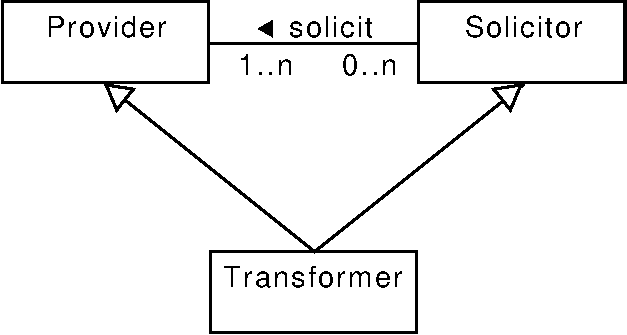
\includegraphics[width=0.5\textwidth]{cpsp_class_diag-crop}
\caption{class diagram of the Provider-Solicitor modeling}
\label{cpsp_class_diag}
\end{figure}

It is important to understand that an agent is not limited to one role only. For a given system an agent can, depending on the context, assume any combination of these roles. Thus an agent can both solicit others agents regarding a resource, while providing a controlled resource to others agents.
In this regard, an agent can even be a producer and solicitor of the same resource. For example the agent is in charge of a specific resource, but also benefit from it. In this case the agent can possibly be in conflict with others agents regarding the state of the resource, and decide (as a producer) to go against its own interest (as a solicitor) in order to help another agent deemed more important.
Obviously, in most implementations, the different roles of the agent would not be as much segregated, and the agent would not strictly communicate with itself using message-passing. This distinction should not be a problem in practice (this kind of configuration can however trigger others CPSP, see for example [[Asynchronous Requests]]).

\subsection{Problem Pattern}

[[Name, Description, Minimal Form, Alternates forms, Symptoms, Solution(s)]]

\subsection{Solution}

\section{Identified Collective Problem Solving Patterns}

In this section, we present the CPSP we identified from the NCS we encountered during the design of our MAS.

\subsection{Conflicting Requests and Criticality}

\subsection{Cooperative Trajectories}

\subsection{Cycle Solving}

\subsection{Hidden Dependencies}

\subsection{Asynchronous Requests}

\section{Conclusion on Collective Problem Solving Patterns}
We identified these patterns from the the NCS of our system. In reverse, the NCS used in the design of AMAS seems perfectly adequate to instantiate known CPSP. Indeed, subsumption-based behavior architectures are appropriate the model this kind of \enquote{exception}-like situations. Should CPSP become more wildly used, one could expect this way of modeling behavior to become quite popular.